\documentclass[conference]{IEEEtran}
\IEEEoverridecommandlockouts
% The preceding line is only needed to identify funding in the first footnote. If that is unneeded, please comment it out.
\usepackage{cite}
\usepackage{amsmath,amssymb,amsfonts}
\usepackage{algorithmic}
\usepackage{graphicx}
\usepackage{textcomp}
\usepackage{xcolor}
\usepackage{algorithmic}
\usepackage{algorithm}
\usepackage{array}
\usepackage[caption=false,font=normalsize,labelfont=sf,textfont=sf]{subfig}
\usepackage{stfloats}
\usepackage{url}
\usepackage{verbatim}
\usepackage[hypcap=false]{caption}
\usepackage{float}
\def\BibTeX{{\rm B\kern-.05em{\sc i\kern-.025em b}\kern-.08em
    T\kern-.1667em\lower.7ex\hbox{E}\kern-.125emX}}

% Set path for images
\graphicspath{ {./images/} }

\newenvironment{Figure}
    {\par\medskip\noindent\minipage{\linewidth}}
    {\endminipage\par\medskip}

\begin{document}

\title{Explainable Machine Learning Guided Modeling for Antennas\\
}

\author{\IEEEauthorblockN{Tyler Carr}
\IEEEauthorblockA{\textit{WiDE Laboratory} \\
\textit{Embry-Riddle Aeronautical University}\\
Daytona Beach, Florida\\
carrt12@my.erau.edu}
\and
\IEEEauthorblockN{Cameron Martinez}
\IEEEauthorblockA{\textit{WiDE Laboratory} \\
\textit{Embry-Riddle Aeronautical University}\\
Daytona Beach, Florida \\
martc114@my.erau.edu}
\and
\IEEEauthorblockN{Dr. Eduardo Rojas-Nastrucci}
\IEEEauthorblockA{\textit{WiDE Laboratory} \\
\textit{Embry-Riddle Aeronautical University}\\
Daytona Beach, Florida \\
rojase1@erau.edu}
\and
\IEEEauthorblockN{Dr. M. Ilhan Akbas}
\IEEEauthorblockA{\textit{WiDE Laboratory} \\
\textit{Embry-Riddle Aeronautical University}\\
Daytona Beach, Florida \\
akbasm@erau.edu}
}

\maketitle

\begin{abstract}
Antenna design processes require extensive electromagnetic (EM) simulation tasks that are resource-intensive, time-consuming, and prone to interruptions. Design equations are only available for predefined and limited antenna geometries. By applying a machine learning (ML) model to a limited set of data from electromagnetic simulations of a leaky wave antenna, performance metrics can be predicted significantly quicker than running simulations for an extensive range of geometric variations. Insights about which geometric parameter had the most significant impact on the prediction can be drawn from the model – hence, explainable ML - and included in the output. The model can be used for inverse design techniques, where the performance requirements are provided as input, and the model generates a geometric solution that meets those requirements. Explainable ML processes can then be applied to analyze which geometric parameter had the largest impact on the performance prediction. The design process was tested on XXX.
\end{abstract}

\begin{IEEEkeywords}
Antennas, machine learning, explainable AI, optimization, regression
\end{IEEEkeywords}


\section{Introduction}

In the realm of wireless communication, microstrip patch antennas have emerged as a favored choice due to their compact size, ease of fabrication, and adaptability to various applications. Comprised of a metallic patch on a dielectric substrate, these antennas offer tunable performance characteristics such as resonant frequency, bandwidth, and radiation pattern. Despite their simplicity, predicting the behavior of microstrip patch antennas involves intricate considerations of parameters like patch dimensions, substrate properties, and feeding mechanisms \cite{Patch_antennas}.

Traditionally, the design and analysis of microstrip patch antennas relied on theoretical models and electromagnetic simulation software, like ANSYS High-Frequency Structure Simulator (HFSS), which necessitates significant computational resources and manual iterations~\cite{john_antenna_2009,ranjan_design_2023,liu_efficient_2014}. However, the integration of machine learning (ML) techniques has revolutionized this process by enabling rapid prediction and optimization of antenna behavior. By leveraging datasets of simulated antenna configurations, ML models can learn complex patterns and relationships, thus streamlining antenna development and enhancing performance in wireless communication systems.

The basic design of this work is a inset-fed microstrip patch antenna, similar to that shown in \cite{inset_feed_pa}. It uses Rogers RT/duroid 5870, with a dielectric constant of 2.33 and dissipation factor of 0.001, for the dielectric substrate layer. There are a few crucial design parameters for the microstrip patch antenna, which are outlined in Figures~\ref{Planar view} and~\ref{3D view}. This design is implemented into HFSS so that it can be modeled and simulated. 

\begin{Figure}
    \centering
    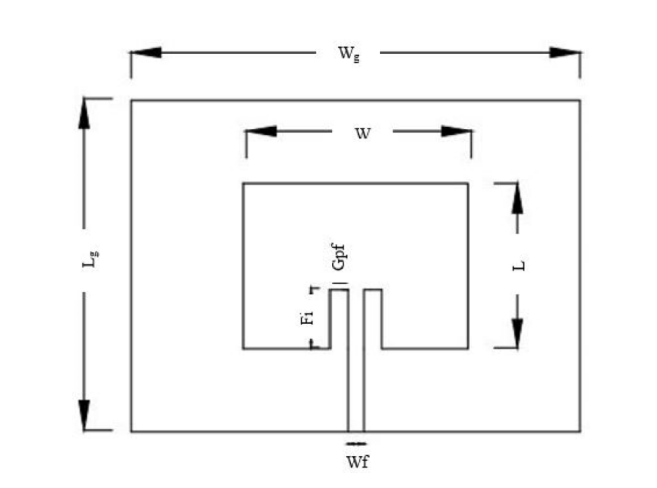
\includegraphics[width=3in]{inset_fed patch antenna.png}
    \captionof{figure}{Planar view of inset-fed patch antenna}
    \label{Planar view}
\end{Figure}


\begin{Figure}
    \centering
    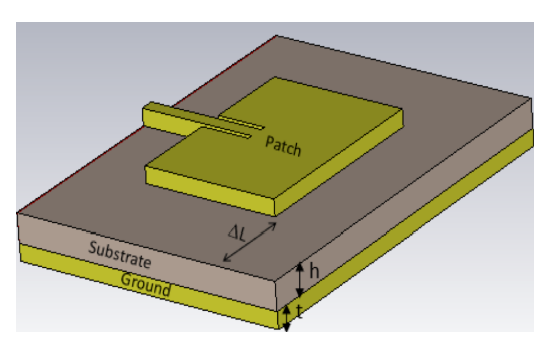
\includegraphics[width=3in]{3D patch antenna.png}
    \captionof{figure}{3-D view of inset-fed patch antenna }
    \label{3D view}
\end{Figure}

One important way to evaluate antenna performance is through its scattering parameters (S-parameters), specifically its $S_{11}$. This is known as the reflection coefficient or return loss, and represents the ratio of input power to reflected power, typically expressed in decibels (dB). For passive systems, this value is always negative. A return loss of less than -10dB demonstrates a high level of impedance matching for an antenna, and is crucial for optimizing antenna performance in terms of signal strength, bandwidth, and radiation efficiency. 

By changing the main antenna design parameters (inset\_dist, L, sub\_thick, W, W0, and y0), a new geometry is created, which generates a new $S_{11}$ response. These geometry specific $S_{11}$ values, along with the parameters of that geometry, were compiled into a dataset, which was then used for training and validating the machine learning model to prove the process works well with a simple antenna design. The dataset consists of 23,735 rows, which was comprised of 233 unique geometries with $S_{11}$ values simulated across 101 frequency range values between 11GHz and 20GHz. Table~\ref{antenna_dataset} describes the relationship between the data.


\begin{table}[h]
\caption{Leaky Wave Antenna Dataset}
\begin{center}
\begin{tabular}{ |l|l|l|l| }
    \hline
    Parameter & Min & Max & Step \\ 
    \hline
    cpw\_in [mm] & 1.5 & 2.5 & 0.25 \\
    \hline
    feed\_l [mm] & 3.25 & 4.25 & 0.25 \\
    \hline
    patch\_l [mm] & 3.25 & 4.25 & 0.25 \\
    \hline
    cpw\_g [mm] & 0.12 & 0.36 & 0.06 \\
    \hline
    Feed\_W [mm] & 0.5 & 2.0 & 0.5 \\
    \hline
    ground\_w [mm] & 0.5 & 1.5 & 0.5 \\
    \hline
    patch\_ground\_w [mm] & 0.5 & 1.5 & 0.5 \\
    \hline
    patch\_w [mm] & 4.5 & 5.0 & 0.25 \\
    \hline
    Freq [GHz] & 11.0 & 20.0 & 0.09 \\
    \hline
\end{tabular}
\end{center}
\label{antenna_dataset}
\end{table}

There is a lot of research available on the topic of how different types of models can be useful in antenna design optimization. Liu et al.~and Li et al.~both proposed methods involving an evolutionary search mechanism~\cite{liu_efficient_2014,li_adaptive_2023}. He et al.~combined an ANN with a simulated annealing algorithm of a wideband patch antenna with four geometric parameters~\cite{10318051}. There are various other papers that compared the $R^2$ and RMSE scores of different regression models on a variety of antennas, such as an ultra-wideband, dual-port multi-in multi-out (MIMO), and THz antennas. These models include Decision Tree, Random Forest, XGBoost, K-nearest neighbors (KNN), Lasso, ridge, support vector, and ANN. Most found that KNN algorithm performed the best, and one found that Random Forest was the best~\cite{9119820,ranjan_ultra-wideband_2022,ranjan_design_2023,sharma_machine_2020,jain_estimation_2022,jain_design_2024}. The above examples have proven that applying machine learning to antenna geometry optimization can decrease both the amount of time taken and the computational expensiveness when compared to typical EM simulations.

There has been less research performed with the intention of reversing the dataset and receiving optimized geometry parameters from specified desired antenna performance values. However, all of the research found appears to follow the same pattern of reversing the inputs and outputs of the respective model, using EM parameters such as gain of $S_{11}$ as inputs and using geometry parameters as outputs. Xiao et al.~applied an inverse extreme learning machine (ELM) and an ANN in an attempt to solve this problem~\cite{9063448,XiaoLi-Ye2021IANN}. Some other methods that were observed were inverse deep neural networks (DNN)~\cite{wu_ai_2024,zhang_inverse_2023}, invertable neural networks~\cite{yu_design_2020}, and more examples of ANNs~\cite{yuan_multibranch_2020}.

This proposed method combines takes a different approach to inverting the problem that allows for an additional layer of explainability. The comparisons between the regression models were taken into consideration upon performing our own comparison. A model was chosen, and instead of achieving an inverse model by reversing the inputs and outputs of the model, predictions were made for a generated dataset, which were then made to be searchable. The goal was to output optimized antenna geometries with explanations when given a $S_{11}$ and frequency range faster, while still achieving a similar result as a more complex model.


\section{Methodology}
Making up the generated dataset that will be searched to find the optimal antenna geometry are all possible combinations of geometries and frequencies, adding up to a total of 327,892 unique geometries. These include the original 233. The simulated $S_{11}$ values were used for the original 233 since they were already given, and predictions were generated for the rest of the geometry and frequency combinations. This new dataset added up to a total of 33,117,092 rows.

In order to determine the optimal antenna geometry, a machine learning model was employed. This model was trained with a supervised learning method using the dataset of simulated data for the leaky wave antenna. This is the model that will be used to make predictions in the simulated dataset.
 
The generated dataset with predictions can be searched by specifying the desired $S_{11}$ value and a frequency range that the antenna should operate within. Antenna geometries that match the search are returned, which saves significant time that would be required to set up and perform additional simulations. When seeking an optimal geometry between a certain frequency range, the geometries that results in the $S_{11}$ with the lowest maximum $S_{11}$ range would be chosen.

\subsection{Metrics}
In order to determine if a $S_{11}$ value was predicted accurately or not, a tolerance was utilized. The tolerance is the maximum deviation from the true value that is allowed, and the prediction is considered accurate if it is within the tolerance. This concept is used when calculating the score of a model~\eqref{eq:tolerance}, with $\epsilon$ being tolerance, $\hat{y_i}$ being the $i$th $S_{11}$ prediction, $y_i$ being the $i$th true $S_{11}$ value, and $n$ being the count of data points. The tolerance is assumed to be one when calculating all scores.

Two other common metrics to compare algorithm performance in addition to the tolerance mentioned above are the $R^2$ score~\eqref{eq:rsquared} and the Root Mean Squared Error (RMSE)~\eqref{eq:rmse}~\cite{shcherbakov_survey_2013}. The $R^2$ score represents how well the regression line fit to the data, and the RMSE represents the difference between the predicted and true values.

\begin{figure}[h]
    \begin{equation}
        \text{Score} = \frac{1}{n} \sum_{i=1}^{n}(\left|\hat{y_i} - y_i\right| \leq \epsilon)
        \label{eq:tolerance}
    \end{equation}
    \begin{equation}
        R^2 = 1 - \frac{\sum_{i}(\hat{y_i} - \bar{y})^2}{\sum_{i}(y_i - \bar{y})^2}
        \label{eq:rsquared}
    \end{equation}
    \begin{equation}
        {RMSE} = \sqrt(\frac{1}{n} \sum_{i=1}^{n}(y_i - \hat{y}_i)^2)
        \label{eq:rmse}
    \end{equation}
    \caption{Evaluation Metrics}
\end{figure}


\subsection{Preprocessing}
Preprocessing needed to be performed on the data features before using them with any model. Firstly, the dataset was split into training and testing sets, with 20\% being reserved for testing and comparing the performance of the models, and the remaining 80\% used to train the models. A standardized scaler was then used to standardize the geometries and frequencies by removing the mean and dividing each value by the standard deviation. This is to ensure the values all have the same scale to improve model performance~\cite{9119820}. 


\subsection{Comparing Models}
Scikit-learn is a popular machine learning library where the typical use case is smaller datasets with feature extraction already having been performed~\cite{scikit-learn}. A regression machine learning model was chosen, as the data labels are numeric. There are a multitude of regression models provided by Scikit-learn. The models that were analyzed in this test were RandomForestRegressor, GradientBoostingRegressor, AdaBoostRegressor, CatBoostRegressor, XGBRegressor, and DecisionTreeRegressor. A randomized search was used to determine the best hyperparameters for the use case of each model. Once the optimization was performed, all of the best models had their performance compared using the same metrics. 

To keep the comparison between the algorithms fair, preprocessing steps were performed in the same way for each model. The same random state was used when splitting the dataset into training and testing portions, to ensure that every model received the same subset of data for training. Additionally, the models were evaluated using the same performance metrics. All of the models were run on an Intel i9-10900X 3.70 GHz CPU with 64 GB RAM to eliminate the possibility of hardware anomalies.


\subsection{Model Performance Analysis}
A manual analysis was performed using a number of random unique antenna geometry configurations for the leaky wave antenna. The geometries selected have never been seen by the simulation or the training set. They then have both their simulated and predicted $S_{11}$ values for the entire frequency range from the HFSS and best chosen model compared. This process is done in order to narrow in on random samples of actual data to check that the model is performing comparably to the simulation software. The geometric parameters of the chosen unseen geometries are recorded in Table~\ref{unseen_geometries}.

\begin{table}[h]
\caption{Unseen Geometry Parameters}
\begin{center}
\begin{tabular}{ |l|l|l|l|l|l|l| }
    \hline
    ID & 1 & 2 & 3 & 4 & 5 & 6 \\
    \hline
    cpw\_in [mm] & 2.5 & 1.75 & 1.75 & 1.75 & 2.5 & 2.5 \\
    \hline
    feed\_l [mm] & 3.25 & 3.25 & 3.5 & 4 & 3.75 & 4 \\
    \hline
    patch\_l [mm] & 3.5 & 3.25 & 3.5 & 4 & 3.75 & 4.25 \\
    \hline
    cpw\_g [mm] & 0.18 & 0.3 & 0.3 & 0.12 & 0.36 & 0.24 \\
    \hline
    Feed\_W [mm] & 1.25 & 0.5 & 1.25 & 1.25 & 0.5 & 1.75 \\
    \hline
    ground\_w [mm] & 0.5 & 0.75 & 1 & 1.25 & 1.5 & 1 \\
    \hline
    patch\_ground\_w [mm] & 0.5 & 1 & 0.5 & 1.5 & 1 & 1.25 \\
    \hline
    patch\_w [mm] & 5 & 5 & 5 & 4.75 & 5 & 4.5 \\
    \hline
\end{tabular}
\end{center}
\label{unseen_geometries}
\end{table}    

% \subsection{Finding Optimal Geometry}
% \begin{Figure}
% \centering
% 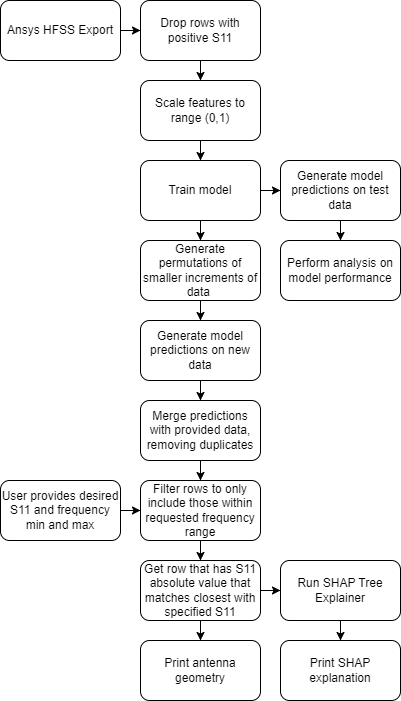
\includegraphics[width=2.5in]{methodology}
% \captionof{figure}{Flow of data through the system}
% \label{data_flow}
% \end{Figure}
% The flowchart in Figure~\ref{data_flow} gives a visual representation of how the data flows through the algorithm. All of the steps up until generating predictions are performed initially for any new antenna configuration that the model hasn't seen yet. The last few steps, starting at filtering rows, are performed every time a new optimal geometry is searched using a specified $S_{11}$ and frequency range. 

% A GUI (graphical user interface) was created in order to make the process of filtering optimal geometries more intuitive. The GUI include an input area, where a user can input a desired $S_{11}$ and frequency range. Once these are entered, all of the combinations are filtered and the best performing optimal geometries are shown. A graph of frequency and predicted $S_{11}$ is also shown, where each optimal geometry is plotted. The desired $S_{11}$ and frequency range are also represented on the graph so it's clear what area of the graph is being focused on.



\subsection{Explainability}
SHAP, an open-source game theoretic approach to explainable AI, is used to demonstrate how much each geometric parameter swayed the predicted $S_{11}$ value~\cite{NIPS2017_7062}. Beeswarm plots are used to enhance understanding of the relationship between the geometric parameters and the $S_{11}$ values by showing which parameters have the highest impact on the prediction being made for the model as a whole, and in which way they are swaying the prediction. By determining which features have the highest impact on the predictions, certain features can be given higher weights in the model to make predictions closer to the simulated values. Waterfall plots can also be created for individual predictions to analyze the highest contributing features to that particular prediction,


\section{Results}
\subsection{Library and Model Comparison}
All of the Scikit-learn regression models had decent accuracies. After performing a randomized search for the best hyperparameters for each model, the score of the best configuration of each model was reported with the $R^2$ and RMSE scores in Table~\ref{comparing_sklearn}. The table is sorted by best to worst performance by score, RMSE, and $R^2$. The goal is to have the accuracy and $R^2$ closest to one, and the RMSE closest to zero. 

It's clear by looking at the table that XGBRegressor is the best performing model. It has the highest accuracy and the lowest RMSE, which proves that its predictions had the least distance from the actual $S_{11}$ values.


\begin{table}[h]
\caption{Scikit-learn Results}
\begin{center}
\begin{tabular}{ |l|l|l|l| }
    \hline
    Model Type & Accuracy within~$\pm$1dB & RMSE & $R^2$ \\ 
    \hline
    XGBRegressor & 0.6271 & 2.686 & 0.7819 \\  
    \hline
    RandomForestRegressor & 0.6164 & 2.613 & 0.7934 \\
    \hline  
    GradientBoostingRegressor & 0.5805 & 2.760 & 0.7697 \\
    \hline
    DecisionTreeRegressor & 0.5123 & 3.276 & 0.6754 \\  
    \hline
    CatBoostRegressor & 0.3691 & 3.369 & 0.6567 \\    
    \hline
    AdaBoostRegressor & 0.3461 & 3.665 & 0.5938 \\  
    \hline
\end{tabular}
\end{center}
\label{comparing_sklearn}
\end{table}

The chosen model was given a set of six random geometries from the leaky wave antenna that were new to both the training and testing sets. These unseen geometries were run through both the HFSS and the chosen machine learning model in order to obtain simulated and predicted $S_{11}$ values for the entire frequency range of the antenna. The results are shown in Figure~\ref{unseen_geometries_graph}, where each unseen geometry has its simulated $S_{11}$ values plotted alongside the predicted values. For all geometries tested, the predicted $S_{11}$ values appear to follow the same trend as the simulated values, but they never reach as far low as the simulated values go. The predictions of the $S_{11}$ values of Geometry 2 were nearly identical to the simulated values. It's interesting to note how for Geometries 3, 4, and 6, both the predicted values and the simulated values had similar dips in the curves around 7GHz and 11GHz. However, the dips were shifted to slightly lower frequency ranges for the predicted values.


\subsection{Testing with Unseen Geometries}
\begin{Figure}
    \centering
    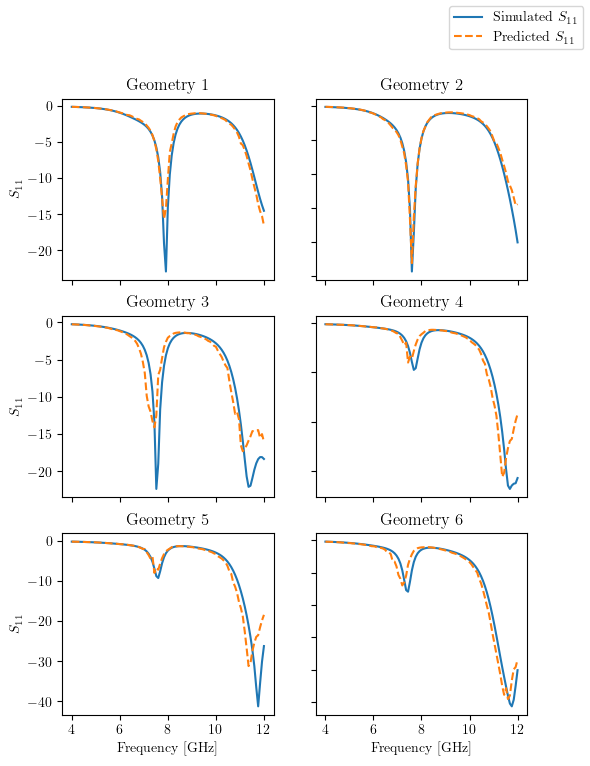
\includegraphics[width=3.5in]{unseen_geometries_freq_vs_seq}
    \captionof{figure}{Simulated \& Predicted $S_{11}$ Values for Frequency Range of Unseen Geometries}
    \label{unseen_geometries_graph}
\end{Figure}

%It's worth noting that each of the geometric parameters that were chosen for the unseen geometries lay within the range of the minimum and maximum value for each respective parameter. Due to the scaling that was performed during the preprocessing steps, any predictions made with geometric parameters that lay outside of the original range of the training data are capped as if the data point outside of the range was actually the corresponding minimum or maximum. 




\subsection{Finding Optimal Geometry}
A graphical user interface (GUI) was implemented using Jupyter Widgets to allow for ease of exploring different types of geometries~\cite{interactive_Jupyter_widgets}. A user inputs a desired $S_{11}$ value and frequency range, and a graph showing predicted $S_{11}$ values for the frequency range will be plotted for the best performing geometries. This graph includes marker lines as a visual aid to show what value the $S_{11}$ predictions should be below and what frequency values the predictions should be between. The GUI allows the user to interactively explore which geometric parameters lead to a specified performance, where before this was a manual and timely process.  


An example of an input and the corresponding graph that is generated is shown in Figure~\ref{gui}. The specified $S_{11}$ value of -25dB is represented by the dotted horizontal blue line, and the selected frequency range between 12.81GHz and 13.03GHz is represented by the two dotted vertical green lines. All of the 4 geometries that are found have predicted $S_{11}$ values within these constraints. Table~\ref{gui_geometries} shows the 4 optimal geometries that are represented in Figure~\ref{gui}. The geometries that are best for this criteria have a $feed\_l$ of 3.75mm and a $patch\_l$ of 4.0mm. The rest of the geometric parameters vary. 

\begin{Figure}
    \centering
    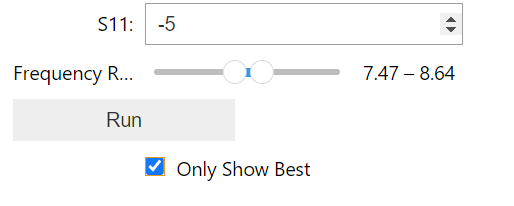
\includegraphics[width=2in]{gui_input}
    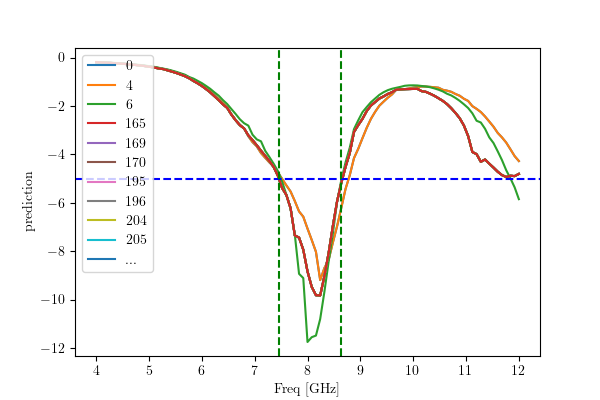
\includegraphics[width=3in]{gui_graph}
    \captionof{figure}{GUI Input and Predicted $S_{11}$ vs Frequency for Optimal Geometries}
    \label{gui}
\end{Figure}

\begin{table}[h]
\caption{Geometries Generated from GUI}
\begin{center}
\begin{tabular}{ 
|p{1.75cm}|p{1cm}|p{1cm}|p{1cm}|p{1cm}|p{1cm}|}
    \hline
    ID & 17505219 & 17528247 & 17528348 & 17535822 & 17543397 \\
    \hline
    cpw\_in [mm] & 2.00 & 2.00 & 2.00 & 2.00 & 2.00 \\
    \hline
    feed\_l [mm] & 4.00 & 4.00 & 4.00 & 4.00 & 4.00 \\
    \hline
    patch\_l [mm] & 3.50 & 3.50 & 3.50 & 3.50 & 3.50 \\
    \hline
    cpw\_g [mm] & 0.18 & 0.18 & 0.18 & 0.18 & 0.18 \\
    \hline
    Feed\_W [mm] & 1.00 & 1.25 & 1.25 & 1.50 & 1.75 \\
    \hline
    ground\_w [mm] & 1.50 & 1.50 & 1.50 & 1.50 & 1.50 \\
    \hline
    patch\_ground\_w [mm] & 1.25 & 1.50 & 1.50 & 1.50 & 1.50 \\
    \hline
    patch\_w [mm] & 4.75 & 4.75 & 4.50 & 4.75 & 4.75 \\
    \hline
\end{tabular}
\end{center}
\label{gui_geometries}
\end{table}   

\subsection{SHAP}
In order to feasibly use SHAP with the patch antenna dataset, a random sample of 5,000 points was used. This sample consisted of all of the geometric parameters and the frequency, and accurately captures characteristics and trends present of the entire dataset. The best performing model, which was XGBRegressor, was used with scaled data in order to interface with the SHAP primary explainer. 

    
\begin{Figure}
\centering
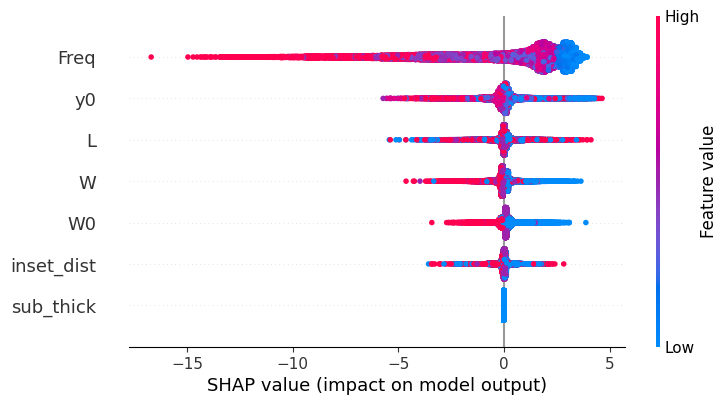
\includegraphics[width=3in]{shap_beeswarm}
\captionof{figure}{Beeswarm Plot of Features Impacting Predictions}
\label{shap_beeswarm}
\end{Figure}

Figure~\ref{shap_beeswarm} is a SHAP beeswarm plot, which is used to demonstrate the impact that each feature had on the predictions made by the model overall. The figure shows how frequency had a significantly higher impact on $S_{11}$ predictions than any geometric feature, and this makes sense when considering that every unique geometry configuration has $S_{11}$ predictions that generally follow the same pattern across the frequency range. All of the other geometric parameters appear to have similar impacts on the predictions being made. $feed\_l$, $ground\_l$, and $Feed\_W$ all very consistently had higher values of these features causing lower predictions to be made, and lower values causing higher predictions. The opposite was true for $cpw\_in$, with most higher feature values causing higher $S_{11}$ predictions. $cpw\_g$ was a bit different than the rest of the features, where high feature values caused both high and low predictions, but lower feature values caused the prediction to stay relatively the same. None of the other features had this strong of a correlation, and appeared to be more randomly distributed. 

\section{Conclusion}
Applying a machine learning algorithm as an aid in the process of optimizing antenna geometric parameters with EM simulations greatly reduces the amount of time and computational power required. Training a model on a small set of data obtained from running simulation software allows the model to fit to the trend of data. Large amounts of additional data can then be generated within the bounds of the existing data, and performance predictions can be made for this generated data with a high accuracy. The most optimal geometries can be returned for specified performance values and frequency ranges, making it unnecessary to run use a trial-and-error process to find these geometries by running simulations. Open-source ML explainability libraries can then be applied to the model and data to allow for further analysis of the contribution each geometric feature makes to the predictions. 

\bibliographystyle{IEEEtran}
\bibliography{refs}


\end{document}
